\documentclass[11pt]{article}
\usepackage{setspace}
\usepackage[a4paper,margin=1in]{geometry}
\geometry{margin=0.85in}
\setstretch{1.0}
\usepackage{graphicx}
\usepackage{array}
\usepackage{setspace}
\usepackage{parskip}
\usepackage{ragged2e}

\pagestyle{empty}
\setstretch{1.0}

\begin{document}


% Title
\begin{center}
    {\Large \textbf{Job Application}} \\[3cm]
    
    {\Huge \textbf{Zhongli Wang}} \\[0.4cm]
    
    {\huge Application for Postdoctoral Researcher}
\end{center}

\vspace{0.6cm}

% Large picture in the middle
\begin{center}
    \IfFileExists{../zhongli-wang-profile.jpg}{
        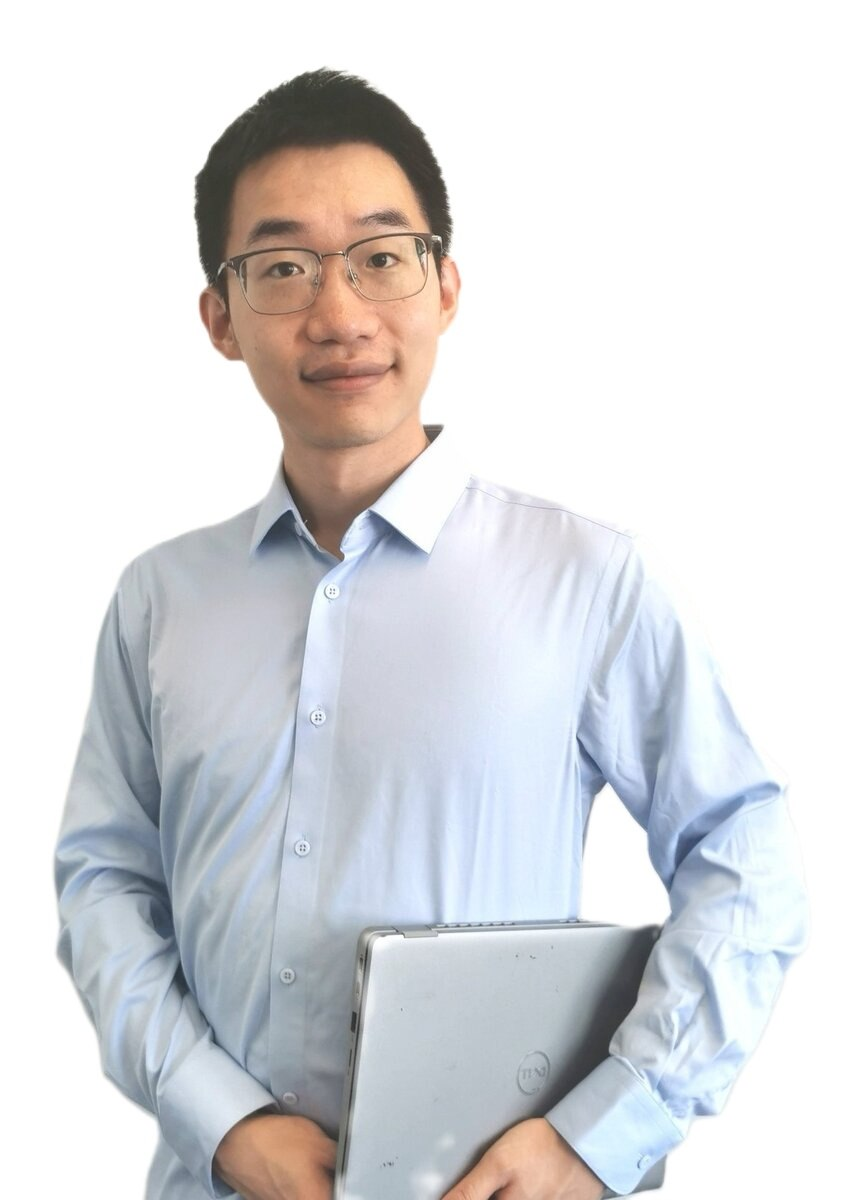
\includegraphics[
            width=0.55\textwidth,
            height=0.45\textheight,
            keepaspectratio
        ]{../zhongli-wang-profile.jpg}
    }{
        \vspace{0.45\textheight}
    }
\end{center}

\vspace{0.7cm}

% \vspace{3cm}


% Personal details
\begin{center}
\renewcommand{\arraystretch}{1.35}
\begin{tabular}{>{\bfseries}p{4.2cm} p{8.5cm}}


Address: & Astastrasse 22, 33617 Bielefeld, Germany \\

Number: & +49 160 9541 6015 \\

Email: & nkwangzhongli@gmail.com \\
\end{tabular}
\end{center}

\vfill

% \begin{center}
%     \small Last updated: \today
% \end{center}
\newpage
\enlargethispage{4\baselineskip}

\begin{flushright}
Zhongli Wang \\
Astastrasse 22 \\
33617 Bielefeld \\
Germany \\
\end{flushright}

\vspace{0.1cm}

\noindent
Prof. Hao (Frank) Yang \\
Department of Civil and Systems Engineering \\
Data Science and AI Institute \\
Johns Hopkins University

\vspace{0.1cm}

\noindent
Application for Postdoctoral Researcher in GenAI and Transportation at the Yang Lab \\

\vspace{0.05cm}

\noindent Dear Prof. Yang,

I am writing to express my interest in the postdoctoral researcher openings in GenAI and Transportation at the Yang Lab. 
I am completing the final stage of my Ph.D. in Economics at Bielefeld University, with my defense scheduled for September 21, 2026, 
and I am currently completing research-related commitments. 
I expect to be available to start work in November 2026. 
My research combines computational modeling, machine learning, AI-assisted workflows, and decision-focused analysis, 
which fits your call for candidates interested in foundation models, AI for decision-making, and computational methods.

Your projects are especially interesting to me because they connect GenAI with real systems problems in traffic safety, transportation planning, and operations. 
Although my doctoral work is not in transportation, it is closely related in method: I build computational models of interacting agents, 
study decision-making under constraints, estimate parameters, and use simulation to understand how system-level outcomes emerge from individual behavior.

My closest fit with the Yang Lab is the ability to move between model design, data analysis, and implementation. 
In my job market paper, I develop an agent-based model of competing ICT firms and analyze how network effects, capacity constraints, and strategic investment shape market outcomes. 
In a published financial fraud detection project, I used accounting, financial, and market indicators with XGBoost to identify red flags in listed companies. 
In another research project, I worked on agentic workflows for economic research using LLMs and multimodal AI, implemented with Microsoft's AutoGen.

I would bring the following strengths to the Yang Lab:

\begin{itemize}
    \item \textbf{GenAI and ML implementation:} Python, XGBoost, scikit-learn, AutoGen, LangChain, OpenAI API, and reproducible research workflows.
    \item \textbf{Decision and systems modeling:} Agent-based modeling, heterogeneous agents, SMM, MCMC, network effects, and constrained strategic decision-making.
    \item \textbf{Research communication:} Experience presenting assumptions, validation choices, and results at international conferences and interdisciplinary workshops.
\end{itemize}

At JHU, I would aim to contribute by adapting foundation-model and agentic-AI methods to decision-support settings, 
building transparent computational pipelines, and testing whether model outputs are useful for planning and operational decisions. 
I am self-motivated, quick to learn, and comfortable working across economics, machine learning, and systems-oriented research.

Thank you for your time and consideration. 
I would welcome the opportunity to discuss how my background in computational economics, AI workflows, and machine learning 
could contribute to your GenAI and transportation research at Johns Hopkins University.

\vspace{0.05cm}
\noindent Sincerely, \\[0.08cm]
\noindent Zhongli Wang \\[-0.2cm]

\vspace{0.1cm}
\noindent
\includegraphics[width=2.7cm,keepaspectratio]{../Wang-sig.jpg}

\end{document}
